\section{Tahapan Desain}
\label{sec:tahapan-desain}
\begin{figure}[htbp]
    \centering
    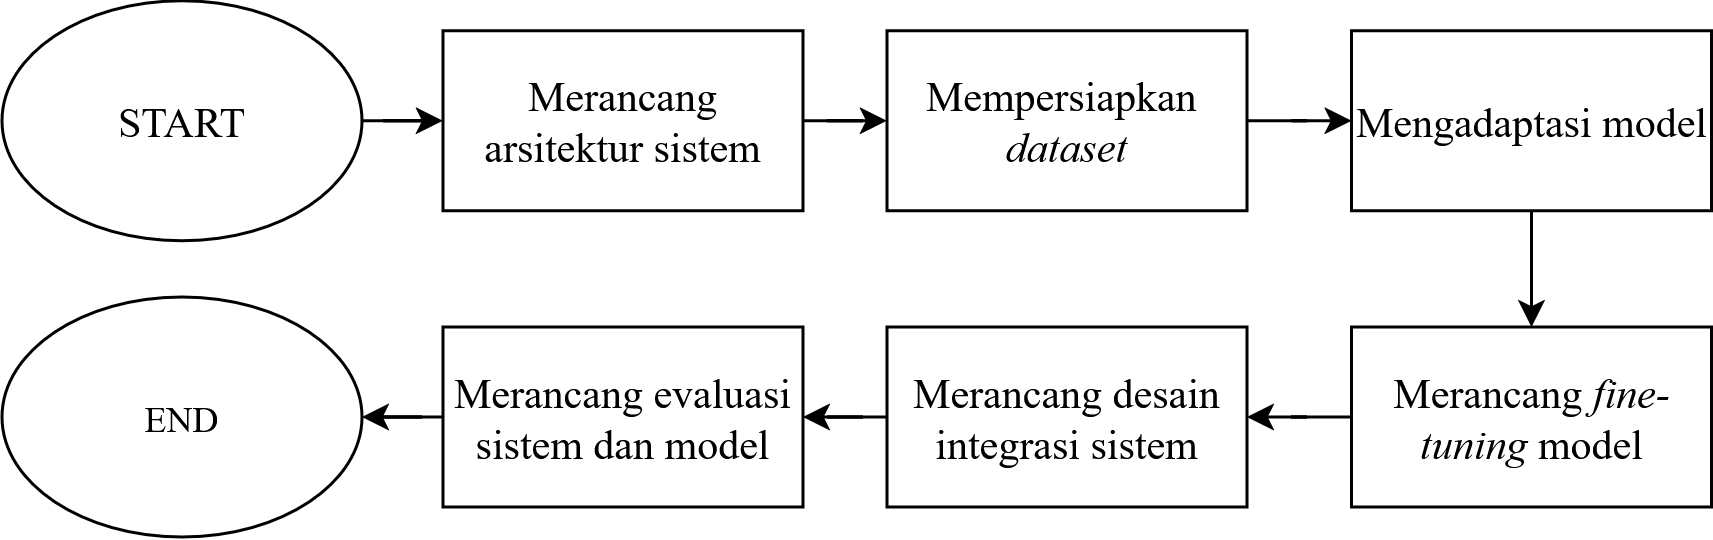
\includegraphics[width=\textwidth]{images/design-flow.png}
    \caption{Alur kerja tahapan desain sistem ekstraksi data struk dan bukti pembayaran}
    \label{fig:design-flow}
\end{figure}

\autoref{fig:design-flow} menunjukkan tahapan desain yang dilakukan dalam penelitian ini. Tahapan desain utama mencakup perancangan \emph{fine-tuning} model, perancangan konversi model, perancangan aplikasi \emph{mobile}, dan perancangan \emph{backend service} sebagai \emph{fallback mechanism}. Tahapan desain yang dihasilkan akan menjadi dasar untuk mengembangkan sistem ekstraksi data struk dan bukti pembayaran. Tahapan desain dirancang berdasarkan pada alternatif solusi yang telah diusulkan pada \autoref{sec:analisis-pemilihan-solusi} dan disesuaikan dengan tahap desain pada metodologi \dsrm.

\subsection{Perancangan \emph{Fine-Tuning} Model \donut}
\label{subsec:perancangan-fine-tuning-model}

Subbab ini menjelaskan rancangan proses \emph{fine-tuning} model \donut{} untuk tugas ekstraksi data bukti pembayaran. Perancangan ini mencakup pemilihan model dasar, konfigurasi arsitektur, desain format keluaran, strategi \emph{preprocessing} data, dan konfigurasi pelatihan untuk melakukan \emph{fine-tuning} model \donut{} pada \dataset{} yang telah dipersiapkan. Proses ini bertujuan untuk menghasilkan model yang mampu melakukan ekstraksi informasi dari bukti pembayaran dengan akurasi tinggi, serta dapat diintegrasikan ke dalam aplikasi \emph{mobile}.

\subsubsection{Pemilihan Model Dasar dan Konfigurasi Awal}
\label{subsubsec:pemilihan-model-dasar}

Model dasar yang dipilih untuk proses \emph{fine-tuning} pada \dataset{} bukti pembayaran QRIS dan transfer adalah model \donut{} yang telah di-\emph{fine-tune} pada \dataset{} CORD-v2 yang telah disediakan oleh naver-cloud-ix. Model tersebut diberi alias \donutcord. Model \donutcord{} dipilih dengan mempertimbangkan faktor-faktor berikut:

\begin{enumerate}
    \item \textbf{\emph{Domain similarity}}: Model \donutcord telah dilatih pada \dataset{} dokumen terstruktur yang memiliki kemiripan dengan struk dan bukti pembayaran dalam hal tata letak dan struktur informasi.
    \item \textbf{Pre-trained capabilities}: Model ini telah memiliki kemampuan dasar dalam memahami dokumen semi-terstruktur, sehingga dapat mempercepat proses konvergensi selama \emph{fine-tuning}.
    \item \textbf{Arsitektur optimal}: Kombinasi \swin{} \transformer{} sebagai \emph{encoder} visual dan \bart{} sebagai \emph{decoder} teks telah terbukti efektif untuk tugas \emph{Visual Document Understanding}.
\end{enumerate}

Konfigurasi awal model melibatkan ekspansi vocabulary tokenizer untuk menambahkan token khusus domain pembayaran. Penulis menambahkan 14 token khusus yang terdiri dari:
\begin{enumerate}
    \item Token pembuka dan penutup untuk setiap \emph{field}
    \begin{enumerate}
    \item \texttt{<s\_total\_amount>}, \texttt{</s\_total\_amount>}
    \item \texttt{<s\_transaction\_time>}, \texttt{</s\_transaction\_time>}
    \item \texttt{<s\_transaction\_identifier>}, \texttt{</s\_transaction\_identifier>}
    \item \texttt{<s\_type>}, \texttt{</s\_type>}
    \item \texttt{<s\_target\_name>}, \texttt{</s\_target\_name>}
    \item \texttt{<s\_application>}, \texttt{</s\_application>}
    \end{enumerate}
    \item Token \emph{task identifier}~\\ \texttt{<s\_payment\_proof>}, \texttt{</s\_payment\_proof>}
\end{enumerate}

Ekspansi vocabulary ini memerlukan penyesuaian dimensi embedding layer pada decoder dan konfigurasi ulang parameter \texttt{decoder\_start\_token\_id} untuk memastikan model memulai generasi dengan token task yang tepat.

\subsubsection{Desain Format Keluaran Terstruktur}
\label{subsubsec:desain-format-keluaran}

Penulis merancang format keluaran terstruktur yang memungkinkan ekstraksi informasi yang konsisten dan dapat diparsing secara otomatis. Format yang dirancang menggunakan markup berbasis XML dengan struktur hierarkis sebagai berikut:

\begin{verbatim}
<s_payment_proof>
<s_total_amount>nilai_total</s_total_amount>
<s_transaction_time>waktu_transaksi</s_transaction_time>
<s_transaction_identifier>id_transaksi</s_transaction_identifier>
<s_type>jenis_transaksi</s_type>
<s_target_name>nama_tujuan</s_target_name>
<s_application>aplikasi_pembayaran</s_application>
</s_payment_proof>
\end{verbatim}

Desain ini memiliki beberapa keunggulan:
\begin{enumerate}
    \item \textbf{Struktur yang jelas}: Setiap field memiliki delimiter yang eksplisit, memudahkan parsing dan validasi keluaran.
    \item \textbf{Fleksibilitas}: Field yang tidak terdeteksi dapat diabaikan tanpa merusak struktur keseluruhan.
    \item \textbf{Konsistensi}: Format yang tetap memungkinkan evaluasi otomatis dan sistem monitoring.
    \item \textbf{Extensibility}: Struktur dapat diperluas untuk menambahkan field baru tanpa mengubah parser yang ada.
\end{enumerate}

Token \texttt{<s\_payment\_proof>} berfungsi sebagai task prompt yang memberikan konteks kepada model bahwa tugas yang dijalankan adalah ekstraksi informasi dari dokumen pembayaran, berbeda dari tugas lain seperti ekstraksi dokumen umum.

\subsubsection{Strategi Preprocessing Data}
\label{subsubsec:strategi-preprocessing-data}

Mengingat karakteristik data metadata yang berpotensi mengalami korupsi atau format yang tidak konsisten, penulis merancang strategi preprocessing yang robust dengan beberapa tahapan:

\paragraph{Pembersihan Metadata}
Penulis mengimplementasikan parser multi-tahap untuk menangani file metadata yang berformat JSONL tetapi mengalami masalah formatting:
\begin{enumerate}
    \item \textbf{Parser Array JSON}: Mencoba parsing sebagai array JSON lengkap setelah menambahkan delimiter koma.
    \item \textbf{Parser Line-by-Line}: Jika gagal, melakukan parsing objek JSON per baris dengan tracking brace count untuk rekonstruksi objek yang terpisah.
    \item \textbf{Error Recovery}: Menangani karakter khusus dan trailing commas yang dapat menyebabkan parsing error.
\end{enumerate}

\paragraph{Pencocokan File Gambar}
Sistem pencarian file gambar yang fleksibel diimplementasikan untuk mengatasi inkonsistensi penamaan file:
\begin{itemize}
    \item Pencocokan direct path
    \item Pencocokan case-insensitive untuk handling variasi kapitalisasi
    \item Pencocokan dengan berbagai ekstensi gambar (.jpg, .jpeg, .png)
    \item Pencocokan partial untuk nama file tanpa ekstensi
\end{itemize}

\paragraph{Validasi dan Pembersihan Data}
Setiap sample data divalidasi untuk memastikan:
\begin{itemize}
    \item Keberadaan file gambar yang valid
    \item Kelengkapan ground truth annotation
    \item Konsistensi format field value (normalisasi spasi internal)
    \item Handling nilai null atau kosong
\end{itemize}

\subsubsection{Konfigurasi Pelatihan dan Optimisasi}
\label{subsubsec:konfigurasi-pelatihan}

Penulis merancang konfigurasi pelatihan yang mempertimbangkan keterbatasan sumber daya komputasi sambil memaksimalkan kualitas hasil \emph{fine-tuning}:

\paragraph{Hyperparameter Selection}
\begin{itemize}
    \item \textbf{Learning Rate}: 3e-5, dipilih sebagai trade-off antara kecepatan konvergensi dan stabilitas pelatihan
    \item \textbf{Batch Size}: 1 per device dengan gradient accumulation 8 steps, memberikan effective batch size 8
    \item \textbf{Epochs}: 40 dengan early stopping patience 3 untuk mencegah overfitting
    \item \textbf{Weight Decay}: 0.01 untuk regularisasi model
\end{itemize}

\paragraph{Optimisasi Memori}
Untuk mengatasi keterbatasan memori GPU, penulis mengimplementasikan beberapa teknik optimisasi:
\begin{enumerate}
    \item \textbf{Mixed Precision Training}: Menggunakan FP16 untuk mengurangi penggunaan memori hingga 50\%
    \item \textbf{Gradient Checkpointing}: Menukar komputasi tambahan dengan penghematan memori
    \item \textbf{Memory Management}: Disable pin memory dan multiprocessing pada dataloader
    \item \textbf{Garbage Collection}: Pembersihan cache CUDA secara eksplisit
\end{enumerate}

\paragraph{Data Collation Strategy}
Penulis merancang custom collation function yang menangani:
\begin{itemize}
    \item Forcing decoder input dengan task start token
    \item Proper label masking untuk padding tokens (-100 untuk ignore dalam loss calculation)
    \item Batch consistency handling untuk samples dengan ukuran berbeda
\end{itemize}

\subsubsection{Desain Sistem Evaluasi dan Monitoring}
\label{subsubsec:desain-evaluasi-monitoring}

Sistem evaluasi dirancang untuk memberikan insight mendalam tentang performa model pada level field individual maupun keseluruhan:

\paragraph{Metrik Evaluasi}
\begin{enumerate}
    \item \textbf{Field-wise Accuracy}: Akurasi ekstraksi untuk setiap field secara terpisah menggunakan regex parsing
    \item \textbf{Overall Sequence Accuracy}: Persentase prediksi yang tepat secara keseluruhan
    \item \textbf{Partial Match Analysis}: Evaluasi komponen-komponen yang benar meskipun keseluruhan prediksi salah
\end{enumerate}

\paragraph{Real-time Monitoring}
Penulis mengimplementasikan callback monitoring yang memberikan feedback real-time:
\begin{itemize}
    \item Sample prediction display setiap 5 epoch
    \item Progress tracking dengan tqdm integration
    \item Automatic model evaluation pada akhir setiap epoch
    \item Best model saving berdasarkan validation loss
\end{itemize}

\paragraph{Prediction Post-processing}
Sistem pembersihan output yang menangani:
\begin{itemize}
    \item Duplikasi start tokens
    \item Spasi berlebih dalam field values
    \item Normalisasi format output untuk konsistensi
\end{itemize}

\subsubsection{Strategi Robustness dan Generalisasi}
\label{subsubsec:strategi-robustness}

Untuk meningkatkan kemampuan generalisasi model pada berbagai variasi dokumen pembayaran, penulis merancang beberapa strategi:

\paragraph{Error Handling Mechanism}
\begin{enumerate}
    \item \textbf{Graceful Degradation}: Jika sample mengalami error processing, sistem menggunakan dummy sample untuk menjaga training continuity
    \item \textbf{Tokenization Safety}: Validasi range token ID untuk mencegah out-of-vocabulary errors
    \item \textbf{Decode Error Recovery}: Safe decoding dengan fallback ke empty string untuk token yang tidak valid
\end{enumerate}

\paragraph{Data Quality Assurance}
\begin{itemize}
    \item Filtering sample dengan ground truth yang tidak lengkap
    \item Validasi format gambar dan konversi otomatis ke RGB
    \item Normalisasi nilai field untuk konsistensi (handling numerical values, date formats)
\end{itemize}

\paragraph{Generation Configuration}
Konfigurasi generation yang dioptimalkan untuk task-specific requirements:
\begin{itemize}
    \item \textbf{Beam Search}: Menggunakan 4 beams untuk balance antara quality dan speed
    \item \textbf{Length Control}: Max length 512 tokens dengan early stopping
    \item \textbf{Repetition Prevention}: N-gram repetition penalty dan bad words filtering
    \item \textbf{Token Constraints}: Proper EOS dan padding token handling
\end{itemize}

Rancangan \emph{fine-tuning} ini dirancang untuk menghasilkan model yang robust, akurat, dan dapat diandalkan untuk ekstraksi informasi dari berbagai jenis struk dan bukti pembayaran yang umum digunakan di Indonesia. Implementasi yang telah dirancang akan dijelaskan lebih lanjut pada \autoref{subsec:fine-tuned-model}.

\subsection{Perancangan Konversi dan Kompresi Model}
\label{subsec:perancangan-konversi-dan-kompresi-model}

 Proses konversi dan kompresi model \donut{} dari format PyTorch \emph{orisinil} ke format yang \emph{optimized} untuk \emph{on-device inference}. Proses tersebut diperlukan untuk mencapai tujuan model yang dapat digunakan pada perangkat \emph{mobile} Android. Subbab ini menjelaskan pendekatan yang digunakan untuk konversi model ke format \emph{Open Neural Network Exchange} (ONNX) dan strategi kompresi yang akan diterapkan pada model.

\subsubsection{Perancangan Konversi dan Kompresi Model \donut{} ke ONNX}
\label{subsubsec:strategi-konversi-onnx}

\emph{Open Neural Network Exchange} (ONNX) dipilih sebagai target format konversi utama karena memberikan keunggulan dalam hal portabilitas lintas \emph{platform} dan optimasi \emph{inference}. ONNX menyediakan dukungan luas untuk berbagai \emph{framework} dan perangkat keras, sehingga memungkinkan integrasi yang lebih baik dengan \emph{platform mobile}. Perubahan format menuju \onnx{} merupakan langkah penting untuk memastikan model dapat dioptimalkan.

Arsitektur model \donut{} yang berbasis \textit{VisionEncoderDecoderModel} bukan merupakan arsitektur yang umum untuk dikonversi, sehingga konversi ke ONNX memerlukan pendekatan yang lebih kompleks dibandingkan model lainnya. \onnx{} telah menyediakan \emph{export tool}{}\footnote{\url{https://huggingface.co/spaces/onnx/export}} yang dapat digunakan untuk mengonversi model PyTorch ke format ONNX. \emph{Export tool} ini akan digunakan untuk melakukan konversi model \donut{} ke format ONNX dan model tersebut yang akan digunakan sebagai dasar untuk kompresi model lebih lanjut. 

\subsubsection{Strategi Kompresi dan Kuantisasi Model}
\label{subsubsec:strategi-kompresi-dan-kuantisasi-model}

Model \donut{} yang telah dikonversi ke format \onnx{} akan melalui tahap kompresi untuk mengurangi ukuran model dan meningkatkan kecepatan inferensi pada perangkat mobile. Kompresi ini penting untuk memastikan model dapat berjalan efisien pada perangkat dengan keterbatasan sumber daya, seperti pada perangkat Android. Metode yang digunakan untuk kompresi dan kuantisasi adalah \emph{Dynamic Quantization}. \emph{Dynamic quantization} dipilih sebagai pendekatan utama untuk melakukan kompresi dan kuantisasi model \donut. Metode \emph{Dynamic Quantization} yang dapat diterapkan adalah FP16, INT8, dan UINT8. Pendekatan ini memungkinkan model untuk tetap mempertahankan akurasi yang tinggi sambil mengurangi ukuran model secara signifikan.


\subsection{Perancangan Evaluasi Model}
\label{subsec:perancangan-evaluasi-model}

\subsection{Perancangan \emph{Backend Service} sebagai \emph{Fallback Mechanism}}
\label{subsec:perancangan-fallback-mechanism}   

\subsection{Perancangan Aplikasi \emph{Mobile}}
\label{subsec:perancangan-aplikasi-mobile}

